The experiments of Section \XXX involve several numerical algorithms for solving traffic assignment problems. These all follow the generic iteration depicted in Figure \ref{fig:iteartion}. In the figure, the top block represents function $F$, which maps candidate demand assignments $h^k$ into path costs $c^k$. The bottom block is a solver update function $U$, which updates the candidate assignment based on information from previous iterations. The index $k$ is incremented in each iteration, and the process continues until convergence is reached.

The numerical algorithms use the
\textit{all-or-nothing assignment at iteration $k$}, denoted with $y^k$,
which is obtained by placing all of the demand for each OD pair $w$ onto
paths whose entry in $c^k$ is minimum amongst paths in $\mathcal{P}_w$.
To express this mathematically, we introduce the notation $c^k_p$ for the
cost on path $p$ at iteration $k$, $c^k_w=\{c^k_p\}_{p\in\mathcal{P}_w}$,
and $y^k_p$ for the demand on path $p$ in the all-or-nothing assignment. Then,
\begin{equation}
\label{eq:allornothing}
y^k_p = \left\{
\begin{tabular}{ll}
$d_w/s$ & $p\in\underset{p'\in\mathcal{P}_w}{\text{argmin }} c^k_{p'} $ \\
0 & otherwise
\end{tabular}
\right.
\end{equation}
Here $s$ is the size of the set $\underset{p'\in\mathcal{P}_w}{\text{argmin }} c^k_{p'}$.

\begin{figure}[h]
    \centering
    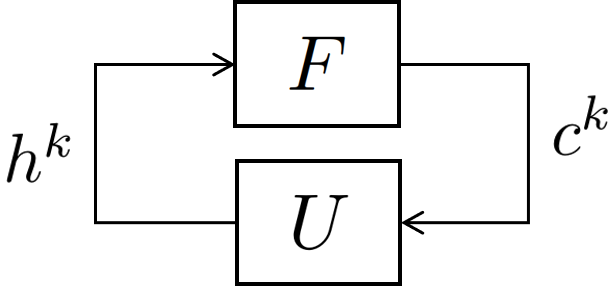
\includegraphics[width=0.4\linewidth]{figs/iteration.png}
    \caption{Generic iteration}
    \label{fig:iteartion}
\end{figure}

\subsection{Frank-Wolfe Algorithm}

The Frank-Wolfe Algorithm (FW) 
\cite{fukushima1984modified,gartner1977analysis} 
is a well-known method for solving convex optimization problems which is especially well suited for network problems. The algorithm has been used in the past to solve large-scale state traffic assignment problems [TTT].

The update function $U$ of FW consists of the following steps:
\begin{enumerate}
\item Compute $y^k$ with Eq. (\ref{eq:allornothing}).
\item Calculate $d^k = y^k - h^k$
\item Calculate the step size $\alpha$ as the solution to the following line-search problem:
\begin{equation}
\begin{aligned}
& \underset{\alpha}{\text{minimize}}
& & F(h^k + \alpha\; d^k)\cdot d^k \\
& \text{subject to}
& & \alpha \in [0,1]
\end{aligned}
\end{equation}
\item $h^{k+1} = h^k +\alpha\; d^k$.
\end{enumerate}

Termination: $c^k(h^k-y^k) \leq \epsilon$

\subsection{Method of Successive Averages}
The Method of Successive Averages (MSA) is a heuristic algorithm for solving variational inequalities. It does not put any restriction on $F$, However it also does not guarantee convergence to a solution  \cite{nie2010solving}.

The update function $U$ of MSA consists of the following steps:
\begin{enumerate}
\item Compute $y^k$ with Eq. (\ref{eq:allornothing}).
\item With step size $\alpha = 1/k$,  $h^{k+1} = (1-\alpha)h^k + \alpha y^k$. 
\end{enumerate}

Terminate if ${\frac {\langle c^k,y^k-h^k \rangle} {\langle y^k, c^k\rangle}} \leq \epsilon$

\subsection{Extra Projection Method}
The Extra Projection Method (EPM) is based on the Euclidean projection operator, defined as,
\begin{equation}
\Pi_\mathcal{H}(x) = \underset{h}{\text{argmin}}\{\lVert h-x\rVert \; : \;h \in\mathcal{H} \}
\end{equation}
where $\lVert\cdot\rVert$ is the Euclidean norm. The EPM guarantees convergence when $F$ is Lipschitz continuous and pseudo-monotone \cite{nie2010solving}. Use $L$ to denote the Lipschitz constant of $F$. $\tau^k$ is a number that should be no larger than $L$.

The update function $U$ of EPM consists of the following steps:

\begin{enumerate}
\item Compute $y^k$ with Eq. (\ref{eq:allornothing}).
\item Find $z^k = \Pi_\mathcal{H}(h^k - \tau^k c^k)$, where $\tau^k < L$ 
\item Evaluate $F(z^k)$.
\item Find $h^{k+1} = \Pi_\mathcal{H}(h^k - \tau^k F(z^k))$
\end{enumerate}
Since $L$ can be difficult to determine in practice, \cite{nie2010solving} proposes the following update equation for $\tau^k$:
\begin{equation}
\tau^{k+1} = \left\{
\begin{tabular}{ll}
$\sigma\;\tau^k$ & 
if $y^{k+1}-y^k < 0$ and $\frac{|y^{k+1}-y^k|}{|y^k|}> \epsilon$ \\
$\tau^k$ & otherwise
\end{tabular}
\right.
\end{equation}


Termination:  If ${\frac {\langle c^k,y^k-h^k \rangle} {\langle y^k, c^k\rangle}} \leq \epsilon$


Here $y^{k+1}$ and $y^k$ are the all-or-nothing assignments corresponding to $h^k$ and $h^{k+1}$ respectively. $\epsilon$ and $\sigma$ are positive scalars between 0 and 1.
